\Titelbanner{9}{Arithmetische \& geometrische Reihen\\
                Der binomische Satz}

\paragraph{Aufgabe 1: } \emph{Arithmetische Reihe}

Wiederholung arithmetische Reihe: $\sum_{k=0}^n (a_0 + k \cdot d) = (n+1)\qty(a_0 + n \frac{d}{2})$ 

\emph{Tafelbeispiel:} 
\begin{itemize}
    \item Summe der ersten $n$ durch fünf teilbaren Zahlen 
    \begin{align}
        0 + 5 + 10 +15 + 20 + \hdots = \sum_{k=0}^n (0+k \cdot 5) = \uuline{\frac{5n(n+1)}{2}}.
    \end{align}
    \item Summe der ersten $n$ ungeraden Zahlen 
    \begin{align}
        \sum_{k=0}^n (2k+1) = (n+1)^2 \qquad (a_0 = 1, d=2).
    \end{align}
\end{itemize}

\emph{Eine Spirale bestehe aus zwei Scharen konzentrischer Halbkreise um die Punkte $A$ und $B$. Es sei $r$ der Radius des innersten Halbkreises und die Strecke $\overline{AB}=e$.}
\begin{enumerate}[label=(\alph*)]\setlength{\itemsep}{-0.5ex}
\item \emph{Wie lang ist der $n$-te Halbbogen?}
\item \emph{Wie lang ist der Gesamtbogen der Spirale bis dahin?}
\end{enumerate}
\begin{figure}[htp]
    \centering
    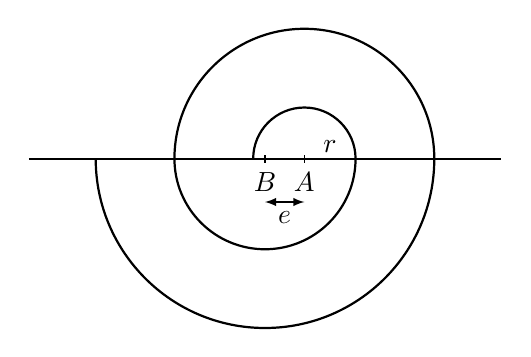
\begin{tikzpicture}[scale=0.5]
        \draw[thick] (-6,0) -- (6,0);
        \draw[thick] (2.3, 0) arc(0:-180:2.3); 
        \draw[thick] (4.3, 0) arc(0:-180:4.3);
        \draw (0,-.1)node[below]{$B$} -- (0,.1); 
        \draw[{latex}-{latex}] (0,-1.1) --node[below]{$e$} (1,-1.1);
        \begin{scope}[shift={(1,0)}]
            \node (A) at (0.65,0.3){$r$};
            \draw (0,-.1)node[below]{$A$} -- (0,.1);
            \draw[thick] (1.3, 0) arc(0:180:1.3); 
            \draw[thick] (3.3, 0) arc(0:180:3.3); 
        \end{scope}
    \end{tikzpicture}
    \vspace{-1.5cm}
\end{figure}

\emph{Lösung:}
\begin{align}
    \begin{rcases}
        \text{1. Halbbogen: } & L_1 = \pi r \\
        \text{2. Halbbogen: } & L_2 = \pi (r+e) \\
        \text{3. Halbbogen: } & L_3 = \pi (r+2e) \\
    \end{rcases} \quad \text{n. Halbbogen:}\quad L_n = \pi r + \pi e (n-1) 
\end{align}
Die Länge der Spirale bis zum $n$-ten Halbbogen: 
\begin{align}
    S_n = \sum_{k=1}^n L_k = n\pi r + \pi e \underbrace{\sum_{k=1}^n k}_{\frac{n\cdot(n+1)}{2}} - n \pi e = n\pi \qty(r + e \frac{n-1}{2}). 
\end{align}
%
\paragraph{Aufgabe 2: } \emph{Geometrische Folge}\\[0.2cm]
\emph{Beim Durchgang durch eine Glasplatte verliert ein Lichtstrahl $\textstyle\frac{1}{12}$ seiner Lichtstärke. Wie viele Platten muss er durchdringen, wenn er nur noch die Hälfte der ursprünglichen Lichtstärke besitzen soll?}\\[0.2cm]
\emph{Hinweis:} \emph{Es genügt die Angabe des Ergebnisses in impliziter Form.}
\begin{itemize}
    \item Lichtstärke nach einem Durchgang: $I_1 = \frac{11}{12} I_0$
    \item Lichtstärke nach $n$ Durchgängen: $I_n = \qty(\frac{11}{12})^n L_0 \overset{!}{=} \frac{1}{2} L_0$
\end{itemize}
\begin{align}
    \Rightarrow \quad n = \frac{\ln(1/2)}{\ln(11/12)} \approx 7.97.
\end{align}
Es müssen also 8 Platten durchdrungen werden, damit der Lichtstrahl auf die Hälfte der Intensität abfällt.
%
\paragraph{Aufgabe 3: } \emph{Geometrische Reihe}

Wiederholung geometrische Reihe: $a_0 \sum_{k=0}^n q^k = a_0\frac{1-q^{n+1}}{1-q}$.
\begin{align}
    \text{Beispiel:} \qquad \sum_{k=0}^n \e^{kx} = \sum_{k=0}^n (\e^x)^k = \uuline{\frac{1-(\e^{x})^{n+1}}{1-\e^{x}}}.
\end{align}

\emph{Es sei eine Anordnung aus zwei Glasplatten gegeben, in die ein Laserstrahl der Intensität $I_\text{in}$ eingeschossen werde. Jede Platte besitze einen Transmissionskoeffizienten $T$ ($0<T<1$), d.h. dass an jeder Platte von einem Lichtstrahl der Intensität $I$ ein Anteil $T\cdot I$ transmittiert und ein Anteil $(1-T)I$ reflektiert wird.
Bestimmen Sie die Intensität $I_\text{out}$, mit der das Licht auf der anderen Seite der Anordnung austritt.}\\
\begin{center}
    \vspace{-1cm}
\begin{tikzpicture}[scale=0.8]
    \node [] at(0.2,0){$I_\text{out}$};
    \draw [<-,line width=0.8pt] (0.7,0)--(2.7,0);
    \draw [line width=1pt] (3.0,-2)--(3.0,2);
    \draw [line width=1pt] (6.0,-2)--(6.0,2);
    \draw [<-,line width=0.8pt] (3.3,0.15)--(5.7,0.15);
    \draw [->,line width=0.8pt] (3.3,-0.15)--(5.7,-0.15);
    \draw [<-,line width=0.8pt] (6.3,0)--(8.3,0);
    \node [] at(8.8,0){$I_\text{in}$};
    \node [below] at(3,-2){$T$};
    \node [below] at(6,-2){$T$};
\end{tikzpicture}
% \vspace{-2cm}
\end{center}
Die Intensität nach $n$-maligem Hinundherlaufen zwischen den Glasplatten (nur austretender Anteil) ergibt sich 
\begin{align}
    \begin{rcases}
        I_0 = T^2 I_\text{in} \\
        I_1 = T^2 (1-T)^2 I_\text{in} \\
        I_2 = T^2 (1-T)^4 I_\text{in}
    \end{rcases} \qquad I_n = T^2 (1-T)^{2n} I_n. 
\end{align}
Die Gesamtintensität am Ausgang ergibt sich aus der Summe der Teilintensitäten: 
\begin{align}
    I_\text{out} &= \sum_{n=0}^\infty I_\text{in} = T^2 I_\text{in} \sum_{n=0}^\infty (1-T)^{2n} \notag \\
    &= T^2 I_\text{in} \lim_{k\to \infty} \sum_{n=0}^k \qty[(1-T)^2]^n = T^2 I_\text{in} \lim_{k\to \infty} \frac{1-\qty[(1-T)^2]^{k+1}}{1-(1-T)^2} \\
    &= T^2 I_\text{in} \frac{1}{1-(1-T)^2} =  \frac{T^2}{2T - T^2} I_\text{in}= \uuline{\frac{T}{2 - T} I_\text{in}}.
\end{align}

\paragraph{Aufgabe 4: } \emph{Der binomische Satz}

\begin{mymathbox}[ams align, title={Binomialkoeffizenten, binomischer Satz}, colframe={FSUblau}]
    \binom{n}{k} &= \frac{n!}{k!(n-k)!} \qq{,} \binom{n}{k} = \binom{n}{n-k} \qq{für} k \le n\\
    (a+b)^n &= \sum_{k=0}^n \binom{n}{k} a^{n-k} b^k \qq{für} a,b \in \mathbb{R}, n\in\mathbb{N}_0
    \end{mymathbox}


\begin{enumerate}[label=(\alph*)]
\item \emph{Berechnen Sie $(1+a)^6+(1-a)^6$}.
Zeichnen wir dazu das Pascal'sche Dreieck 
\begin{figure}[htp]
    \centering
    \begin{tikzpicture}[scale=0.7]
        \foreach{\x} in {0,...,6}{
            \foreach{\y} in {\x,...,6}{
                \pgfmathsetmacro{\binomial}{int(round(factorial(\y)/(factorial(\x)*factorial(\y-\x))))}
            \node at (2*\x-\y,-\y) {$\binomial$};
            } 
        }
        \draw[thick, red, -{latex}] ($(0,-2)+(-.2,-.2)$) -- +(-.6,-.6);
        \draw[thick, red, -{latex}] ($(-2,-2)+(.2,-.2)$) -- +(.6,-.6);
        \draw[thick, PAForange, -{latex}] (-8,-6)node[left]{$n=6$} -- (-6.5,-6);
    \end{tikzpicture}
\end{figure}
Bei der Summe der beiden Terme fallen nun die ungeraden Potenzen von $a$ weg, während die geraden doppelt auftreten.
\begin{align}
    (1\pm a)^6 &= 1 \pm 6a + 15a^2 \pm 20a^3 + 15a^4 \pm 6a^5 + a^6 \\
    \Rightarrow (1+a)^6 + (1-a)^6 &= 2 + 30a^2 + 30 a^4 + 2 a^6.
\end{align}
\item \emph{Schreiben Sie die allgemeine Binomialformel für $(1+x)^n$ und $(1-x)^n$ auf und setzen Sie anschließend $x=1$. In letzterem Falle sei $n\ge 1$.}
\begin{alignat}{3}
    (1+x)^n &= \sum_{k=0}^n \binom{n}{k} x^k \qquad &&\overset{x=1}{\Longrightarrow} \quad \uuline{\sum_{k=0}^n \binom{n}{k} = 2^n} \\
    (1-x)^n &= \sum_{k=0}^n (-1) \binom{n}{k} x^k \qquad &&\overset{x=1}{\Longrightarrow} \quad \uuline{\sum_{k=0}^n (-1)^k\binom{n}{k} = 0}.
\end{alignat}
Das sind nützliche Identitäten im Umgang mit Binomialkoeffizienten. Man veranschauliche sich die Ausdrücke im Pascal'schen Dreieck.
\item \emph{Es seien die Funktionen $f(x)=\left(\e^{x}+\e^{-x}\right)/2$ und $g(x)=\left(\e^{x}-\e^{-x}\right)/2$ definiert. Finden Sie einen Ausdruck, der $f(nx)+g(nx)$, mit $n\in\mathbb{N}$, auf (Potenzen von) $f(x)$ und $g(x)$ zurückführt.}
\begin{align}
    &\begin{rcases}
        f(x) = \frac{1}{2}(\e^{x}+\e^{-x}) \\
        g(x) = \frac{1}{2}(\e^{x}+\e^{-x})
    \end{rcases} \quad \e^{x} = f(x) + g(x) \\
    &\Rightarrow f(nx) + g(nx) = \e^{nx} = (f(x) + g(x))^n = \uuline{\sum_{k=0}^n \binom{n}{k} f(x)^k g(x)^{n-k}}.
\end{align}
Das ist die Formel von Moivre für Hyperbolikus-Funktionen.
\end{enumerate}
%
\paragraph{Aufgabe 5: } \emph{Erzeugende Funktion} \hfill (Zusatzaufgabe)\\[0.2cm]
\emph{Betrachten Sie die Rekursionsgleichung $a_{n+1}=2a_n+1$ mit Anfangswert $a_0=0$ aus Aufgabe 1, Thema 8. Es sei eine (unbekannte) Funktion definiert als}
\begin{align*}
f(x)=\sum\limits_{n=0}^\infty a_n x^n\,.
\end{align*}
\begin{enumerate}[label=(\alph*)]
\item \emph{Multiplizieren Sie beide Seiten der Rekursionsgleichung mit $x^n$, summieren Sie über $n$ (von Null bis Unendlich) ab und versuchen Sie alle auftretenden Terme durch $f(x)$ auszudrücken. Lösen Sie für $f(x)$.}
\begin{align}
    a_{n+1} x^n &= 2 a_n x^n + x^n \\
    \Rightarrow \sum_{n=0}^\infty &= 2 \underbrace{\sum_{n=0}^\infty a_n x^n}_{f(x)} + \underbrace{\sum_{n=0}^\infty x^n}_{\mathrlap{\hspace{-0.3cm}\frac{1}{1-x}, \qq{geometrische Reihe}}} \\
    \Rightarrow \underbrace{\sum_{n=1}^\infty a_n x^{n-1}} &= 2 f(x) + \frac{1}{1-x} \\
    \sum_{n=0}^\infty a_n &x^{n-1} - \cancel{a_0 x^{-1}} = \frac{1}{x} \sum_{n=0}^\infty a_n x^n = \frac{1}{x} f(x) \\
    \Rightarrow f(x) &= 2x f(x) + \frac{x}{1-x} \quad \Rightarrow \quad f(x) = \frac{x}{(1-x)(1-2x)}.
\end{align}
\item \emph{Nutzen Sie Ihr Wissen über geometrische Reihen, um $f(x)$ wieder in Reihendarstellung zu überführen und lesen Sie die Koeffizienten vor $x^n$ ab.}
\begin{align}
    f(x) &= x \underbrace{\frac{1}{(1-x)(1-2x)}}_{\mathclap{\text{Partialbruchzerlegung}}} = x \qty(\frac{\alpha}{1-2x} + \frac{\beta}{1-x})= x \qty(\frac{2}{1-2x}-\frac{1}{1-x}).   \\
    &\quad 1 = \alpha(1-x)+\beta(1-2x) = -x(\alpha+2\beta) + (\alpha+\beta) \\
    &\quad 1 = \alpha + \beta \qq{und} 0 =\alpha + 2\beta  \qquad \Rightarrow \quad \alpha = 2, \beta = -1.
\end{align}
Nun nutzen wir die Ausdrücke für die geometrische Reihe 
\begin{align}
    \frac{1}{1-x} &= \sum_{n=0}^\infty x^n \qq{,} \frac{1}{1-2x} = \sum_{n=0}^\infty (2x)^n \\
    \Rightarrow f(x) &= x(2 \sum_{n=0}^\infty 2^n x^n - \sum_{n=0}^\infty x^n) = x \sum_{n=0}^\infty (2^{n+1} - 1) x^n \\
    &= \sum_{n=1}^\infty (2^n -1) x^n \quad \Rightarrow \quad \uuline{a_n = 2^n -1}.
\end{align}
\end{enumerate}
%
% \paragraph{Aufgabe 6*: } \emph{Zustandssumme}\\[0.2cm]
% Vereinfachen Sie den Ausdruck
% \begin{align*}
% \Omega_N=\sum\limits_{n_1=0}^N\sum\limits_{n_2=0}^N\sum\limits_{n_3=0}^N\dots\sum\limits_{n_k=0}^N f(n_1)f(n_2)f(n_3)\dots f(n_k)\,, \qq{wobei}f(n)=\e^{-n}.
% \end{align*}
% Bestimmen Sie anschließend den Grenzwert $\Omega=\lim\limits_{N\rightarrow\infty}(\Omega_N)$.
% %
% \paragraph{Aufgabe 7*: } \emph{Fibonacci-Zahlen II}\\[0.2cm]
% Wenden Sie das Verfahren aus Aufgabe 5 auf die Folge $a_{n+1}=a_n+a_{n-1}$ der Fibonacci-Zahlen mit Startwerten $a_0=0$, $a_1=1$ an. Beachten Sie, dass hier $n\ge 1$ gelten muss.
%